  %%%%%%%%%%%%%%%%%%%%%%%%%%%%%%%%%%%%%%% -*- coding: utf-8; mode: latex -*- %%
  %
%%%%%                       CHAPTER
 %%%
  %

% $Id: 5100-omnis-voluptas.tex,v 1.1 2007/11/23 09:52:44 david Exp $
% $Log: 5100-omnis-voluptas.tex,v $
% Revision 1.1  2007/11/23 09:52:44  david
% *** empty log message ***
%
%

  %%%%%%%%%%%%%%%%%%%%%%%%%%%%%%%%%%%%%%%%%%%%%%%%%%%%%%%%%%%%%%%%%%%%%%%%%%%%%
  %
%%%%%                    HEAD MATTER
 %%%
  %

\chapter{Evaluation}
%\addcontentsline{lof}{chapter}{\thechapter\quad Nihil Molestiae}
%\addcontentsline{lot}{chapter}{\thechapter\quad Nihil Molestiae}
\label{ch:evaluation}

The solution \textit{Optimistic Concurrency Control with Snapshot Isolation on Semantic Related Group} (OCC) is built on top of the transactional framework~\cite{peiro2013maintaining} in the second version of Hop-HDFS (PCC). The goal is to demonstrate how our OCC solution performs better than PCC. As a proof of concept, we implemented the OCC version for the operation \textit{mkdirs} and give a detailed evaluation compared with PCC in this chapter. For this purpose, we concern about the execution time (elapsed time) needed to finish all the concurrent tasks.

\section{Experimental Testbed}
\label{sec:testbed}

The MySQL Cluster consists of six data nodes connected by 1 Gigabit LAN. Each data node has an Intel Xeon X5660 CPU at 2.80GHz, and contributes 6 GB RAM (5 GB Data Memory + 1 GB Index Memory), therefore, the total available memory for the cluster is 36 GB. The number of data replica is 2. The maximum concurrent transactions is 10000 for each data node, and the inactive timeout for each transaction is 5 seconds. 

\noindent To avoid any communication overhead caused by RPC connections and serialization, we run the NameNode and Clients on the same machine with Intel i7-4770T CPU at 2.50GHz and 16 GB RAM. This machine is connected with the MySQL Cluster data nodes by 100 Megabits LAN.

  %%%%%%%%%%%%%%%%%%%%%%%%%%%%%%%%%%%%%%%%%%%%%%%%%%%%%%%%%%%%%%%%%%%%%%%%%%%%%
  %
%%%%%                      SECOND SECTION
 %%%
  %

\section{Parent Directory Contention Assessment}
\label{sec:ww}

This experiment is the same as described in Section~\ref{sec:pdcassement}, but we expand it to include the results with OCC. See Figure~\ref{fig:hdfsPCCOCCparentDiragram} for the workload visual diagram. Hence, we have a full performance comparison here among HDFS, PCC and OCC (Hop-HDFS).

\begin{figure}[ht]
	\centering
	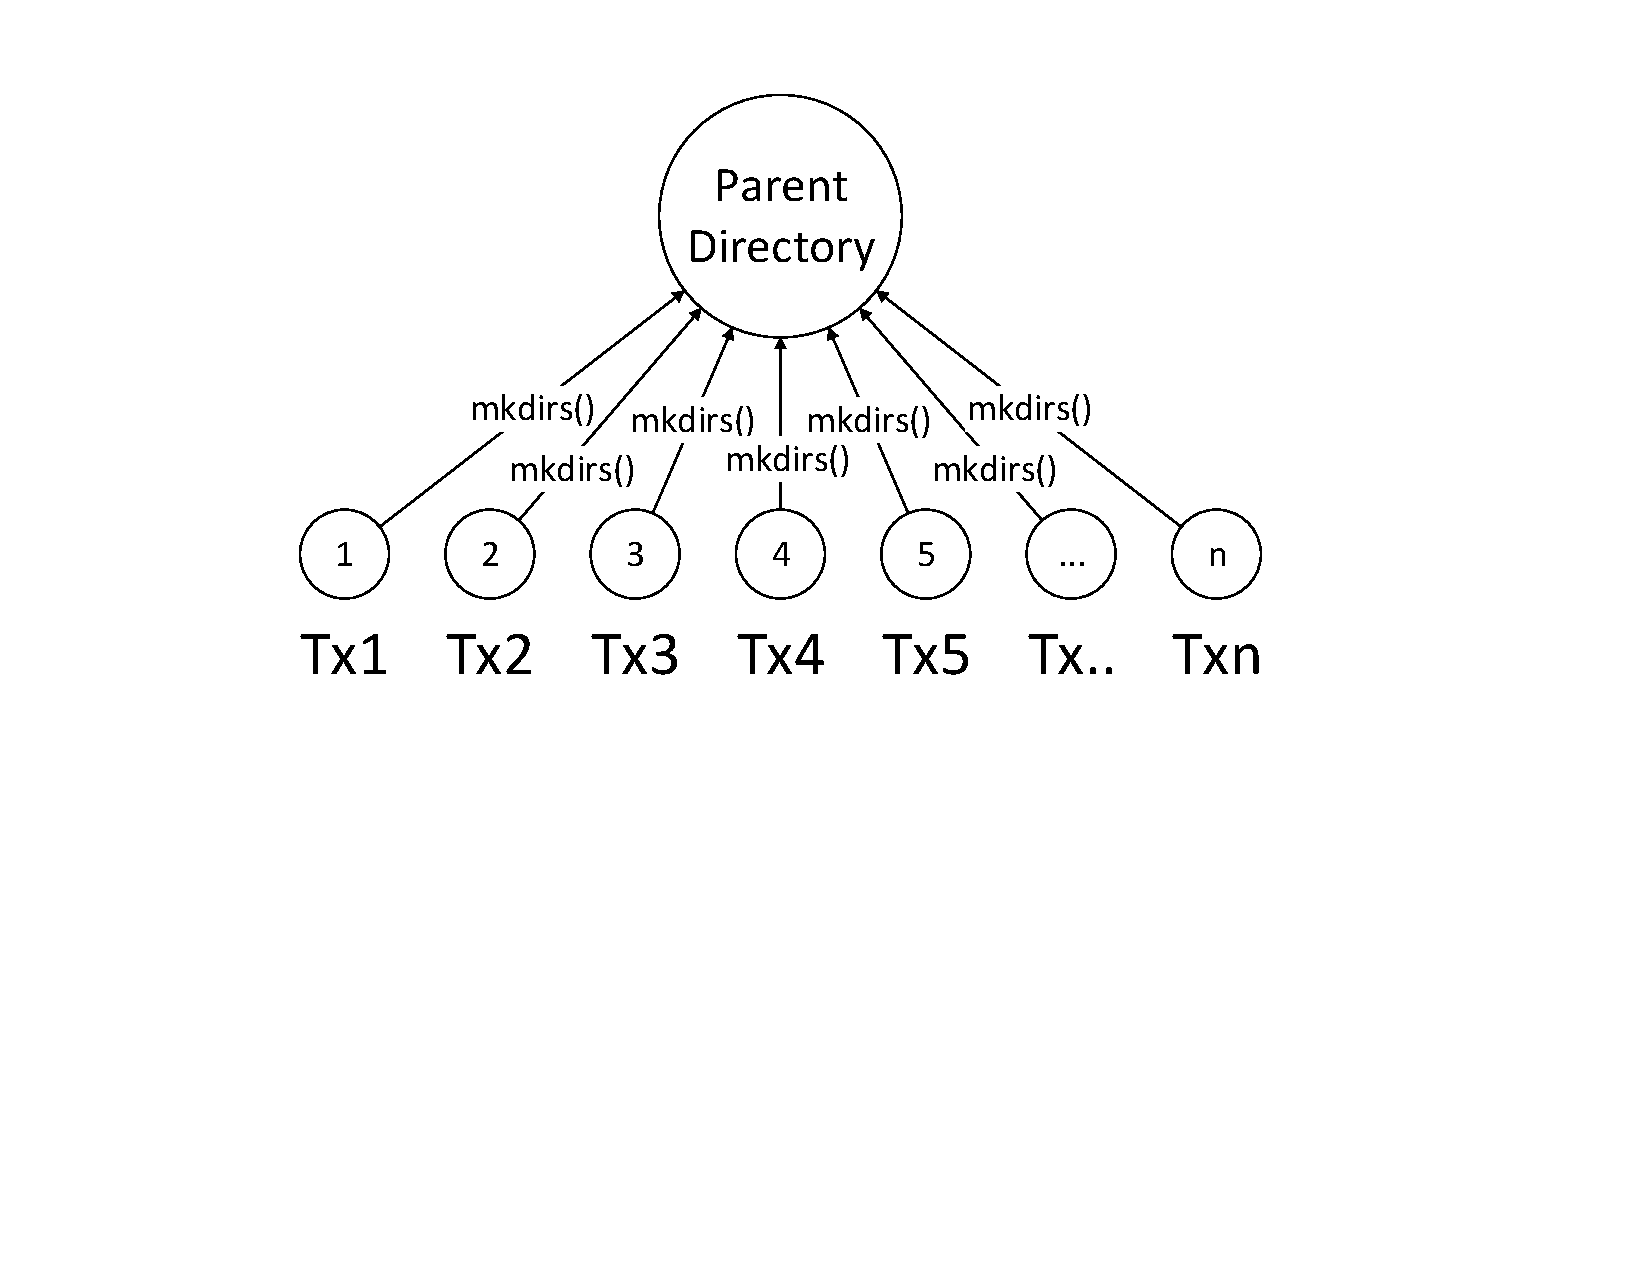
\includegraphics[scale=0.6]{figs/ww.pdf}
	\caption{Workload of Parent Directory Contention Assessment}
	\label{fig:hdfsPCCOCCparentDiragram}
\end{figure}

\noindent From Figure~\ref{fig:hdfsPCCOCCparent} and Table~\ref{fig:hdfsPCCOCCparent}, we can see that OCC significantly outperforms PCC by almost 70 \% on this concurrent write-write parent directory contention workload.

\begin{figure}[ht]
	\centering
	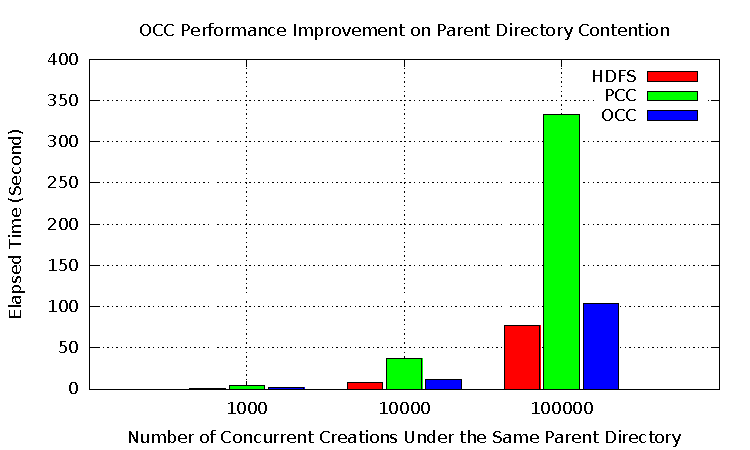
\includegraphics[width=\linewidth]{figs/hdfs_pcc_occ_parent.pdf}
	\caption{OCC Performance Improvement on Parent Directory Contention}
	\label{fig:hdfsPCCOCCparent}
\end{figure}

\begin{table}[ht]
	\centering
	\begin{tabular}{|c|c|c|c|}
		\hline
		\textbf{Num. of Concurrent Creation}                                                 & \textbf{1000}   & \textbf{10000}  & \textbf{100000} \\ \hline
		HDFS                                                                                 & 0.82s           & 7.83s           & 77.13s          \\ \hline
		PCC                                                                                  & 4.35s           & 36.74s          & 332.36s         \\ \hline
		OCC                                                                                  & 1.36s           & 12.01s          & 103.23s         \\ \hline
		PCC / HDFS                                                                           & 530.5\%         & 469.2\%         & 430.9\%         \\ \hline
		OCC / HDFS                                                                           & 165.9\%         & 153.4\%         & 133.8\%         \\ \hline
		\textbf{\begin{tabular}[c]{@{}c@{}}OCC Improvement: \\ (PCC-OCC) / PCC\end{tabular}} & \textbf{68.7\%} & \textbf{67.3\%} & \textbf{68.9\%} \\ \hline
	\end{tabular}
	\caption{OCC Performance Improvement on Parent Directory Contention}
	\label{table:hdfsPCCOCCparent}
\end{table}

\section{Read-Write Mixed Workload Assessment}

In this experiment, we did a test for a read-write mixed workload assessment while the parent directory is still the contention point for PCC and OCC will still outperform in this workload. Similar to the experiment in Section~\ref{sec:ww}, we have 1000, 10000 and 100000 concurrent operations running under the same parent directory. But in each task, half of them will do the metadata read operation \textit{getFileStatus()}, while the other half will do the write operation \textit{mkdirs()}. See Figure~\ref{fig:rwWorkload} for a reference.

\begin{figure}[ht]
	\centering
	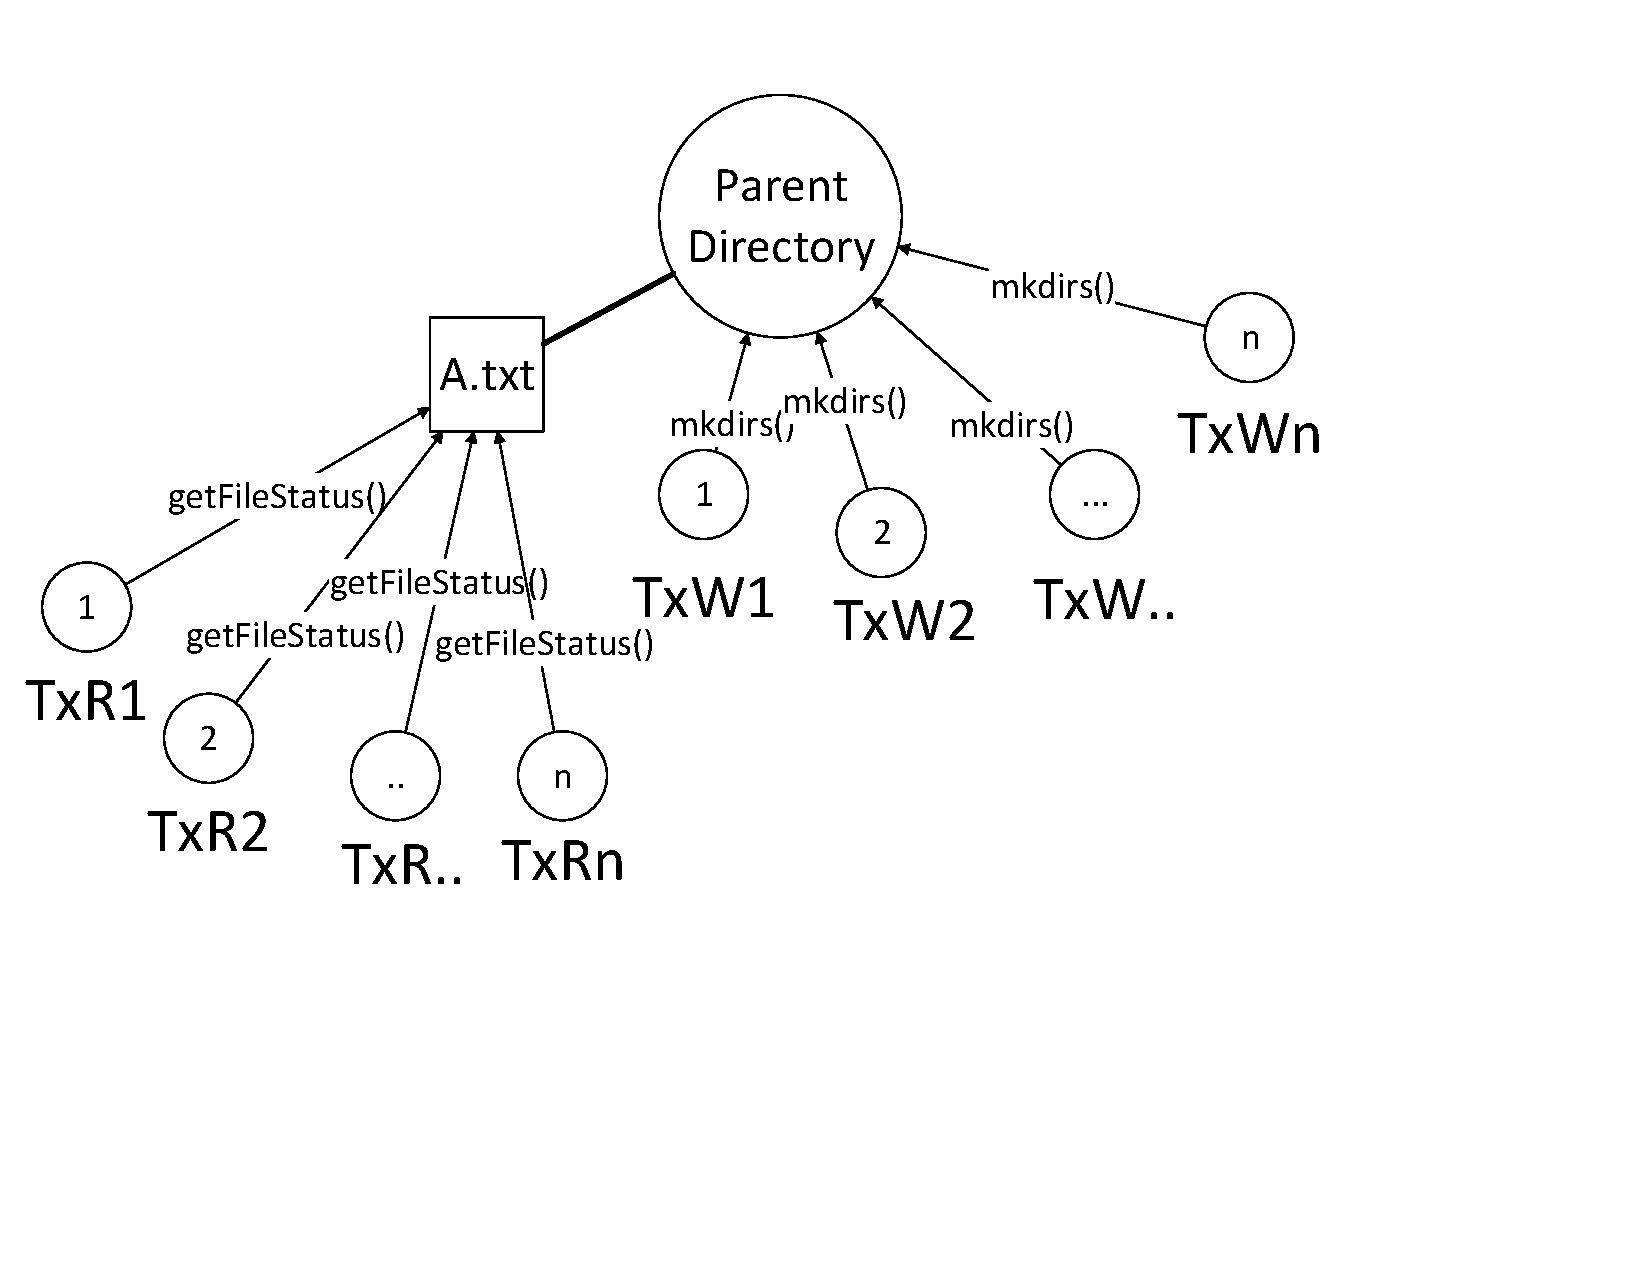
\includegraphics[scale=0.6]{figs/rw.pdf}
	\caption{Read-Write Mixed Workload}
	\label{fig:rwWorkload}
\end{figure}

\noindent From Figure~\ref{fig:rwWorkload} and Table~\ref{fig:rw}, we can see that OCC still significantly outperforms PCC around by 65 \% on this concurrent read-write Mixed Workload. 

\begin{figure}[ht]
	\centering
	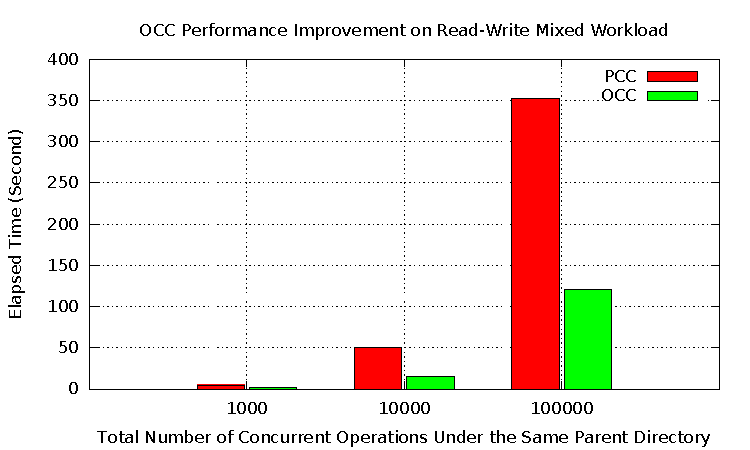
\includegraphics[width=\linewidth]{figs/pcc_occ_rw.pdf}
	\caption{OCC Performance Improvement on Read-Write Mixed Workload}
	\label{fig:rw}
\end{figure}

\begin{table}[ht]
	\centering
	\begin{tabular}{|c|c|c|c|}
		\hline
		\textbf{Num. of Concurrent Creation}                                                 & \textbf{1000}   & \textbf{10000}  & \textbf{100000} \\ \hline
		PCC                                                                                  & 4.92s           & 50.69s          & 352.25s         \\ \hline
		OCC                                                                                  & 1.78s           & 15.31s          & 120.64s         \\ \hline
		\textbf{\begin{tabular}[c]{@{}c@{}}OCC Improvement: \\ (PCC-OCC) / PCC\end{tabular}} & \textbf{63.8\%} & \textbf{69.8\%} & \textbf{65.8\%} \\ \hline
	\end{tabular}
	\caption{OCC Performance Improvement on Read-Write Mixed Workload}
	\label{table:rw}
\end{table}

\section{The Size of Semantic Related Group}

In the read phase and validation phase, we need to fetch the semantic related group from the mutation data. The more levels of directories, the more related rows will be fetch. The depth of the path equals the size of the semantic related group. But since the namespace is a tree structure, in reality, the depth of the namespace won't be too much. HDFS also limit the maximum number of levels to be 1000 and maximum 3000 characters for the whole path. Besides, batch reading is also used to minimize the network round-trips when fetching data. Therefore, the size of semantic related group will not be a big problem in practice. 

\noindent Here we did a test to see how performance affected by different size of semantic related group. Similar to the experiment in Section~\ref{sec:ww}, we have 100 concurrent operations (\textit{mkdirs()}) running under the same parent directory. See Figure~\ref{fig:srg}.

\begin{figure}[ht]
	\centering
	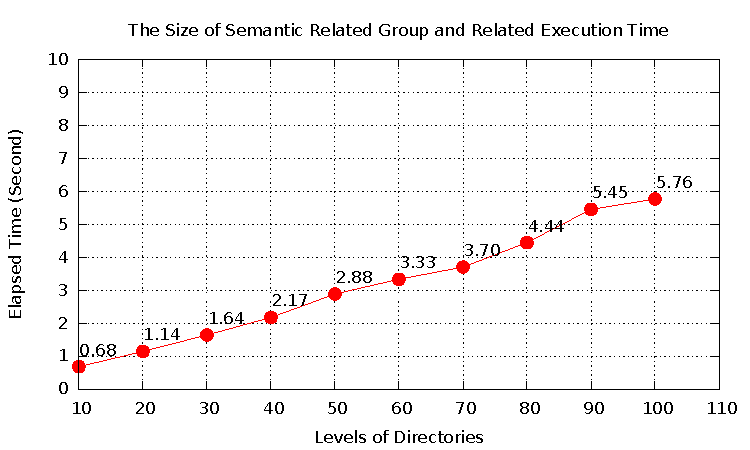
\includegraphics[width=\linewidth]{figs/srgSize.pdf}
	\caption{The Size of Semantic Related Group and Related Execution Time}
	\label{fig:srg}
\end{figure}

\section{OCC Performance with Different Size of Conflicts}

When OCC conflicts happen, transactions will abort, wait for some random time and retry. Eventually one transaction will success and others will read the updated values when retry and return related RPC callbacks to clients.

\noindent Similar to the experiment in Section~\ref{sec:ww}, we have 10000 concurrent operations running under the same parent directory and each operation only creates one sub-directory. But these operations will try to create the same sub-directories in the number of 1 (all conflicts), 10, 100, 1000 and 10000 (no conflicts) separately.

\begin{figure}[ht]
	\centering
	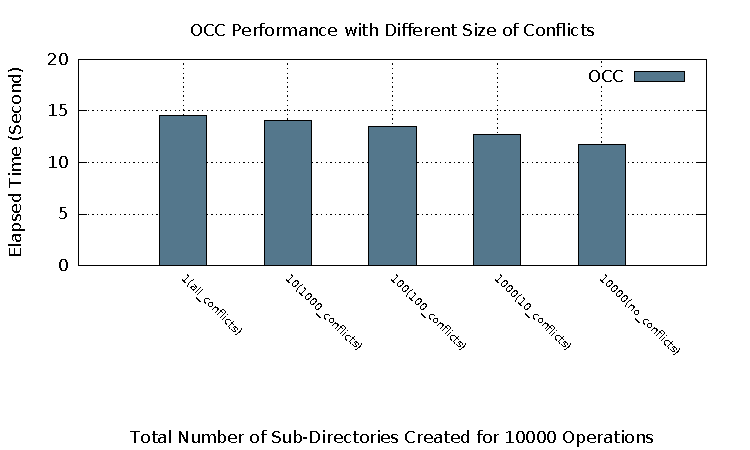
\includegraphics[width=\linewidth]{figs/conflict.pdf}
	\caption{OCC Performance with Different Size of Conflicts}
	\label{fig:conflict}
\end{figure}

\begin{table}[h]
	\centering
\begin{tabular}{|c|c|}
	\hline
	\textbf{Total Num. of Sub-DirectoriesCreated for 10000 Operations} & \textbf{Elapsed Time (Second)} \\ \hline
	1 (all conflicts)                                                  & 14.53                          \\ \hline
	10 (1000 conflicts)                                                & 14.11                          \\ \hline
	100 (100 conflicts)                                                & 13.51                          \\ \hline
	1000 (10 conflicts)                                                & 12.72                          \\ \hline
	10000 (no conflicts)                                               & 11.75                          \\ \hline
\end{tabular}
	\caption{OCC Performance with Different Size of Conflicts}
	\label{table:conflicts}
\end{table}

\noindent From Figure~\ref{fig:rwWorkload} and Table~\ref{fig:rw}, if all operations conflict, the performance degrades by 19.1\%~\footnote{$(14.53-11.75) \div 14.53 = 19.1$\%} for maximum.